
\documentclass[conference]{IEEEtran}

\ifCLASSINFOpdf
  \usepackage[pdftex]{graphicx}
  \graphicspath{{../pdf/}{../jpeg/}}
  \DeclareGraphicsExtensions{.pdf,.jpeg,.png}
\else
\fi

\usepackage{pgfplots}
\usepackage{array}
\usepackage{url}
\usepackage[T1]{fontenc}
\usepackage[utf8]{inputenc}

\hyphenation{op-tical net-works semi-conduc-tor}

\begin{document}

\title{A Survey on the Mathematical Emphasis in Brazilian Computer Science Curricula}

\author{\IEEEauthorblockN{Pedro Paulo Vezzá Campos }
\IEEEauthorblockA{Institute of Mathematics and Statistics\\
University of São Paulo\\
São Paulo, Brazil\\
Email: pedrovc@ime.usp.br}
\and
\IEEEauthorblockN{Jackson José Souza}
\IEEEauthorblockA{Institute of Mathematics and Statistics\\
University of São Paulo\\
São Paulo, Brazil\\
Email: jackson@ime.usp.br}
\and
\IEEEauthorblockN{Giuliano Salcas Olguin}
\IEEEauthorblockA{Faculty of Education\\
University of Campinas\\
Campinas, Brazil\\
Email: giuliano.olguin@gmail.com}}

\maketitle


\begin{abstract}
    A recurring question raised by professors and undergraduate students involves the distribution of basic and pratical - or professional - courses. Some authors defend a curriculum with more basic courses, such as Mathematics, Physics and Chemistry, in order to create a solid background. Moreover, there is a growth of academic exchange programs all around the world, which requires a common learning base.

    Since 1960, the importance of Mathematics in Computer Science (CS) undergraduate curricula has been decreasing, particularly, because new fields in CS have risen and they were assimilated in the curricula. Despite of reduction, Mathematics still have its role in CS's curricula.

    The goal of this paper is to analyze the amount of the courses related to Mathematics in different CS undergraduate curricula. In this work are analyzed the lecture hour load dedicated to Mathematics courses on ten Brazilian CS undergraduate programs: The Federal Universities of Ceará, Minas Gerais, Campina Grande, Pernambuco, Rio de Janeiro, Rio Grande do Sul and Santa Catarina, State Universities of São Paulo and Campinas and the Pontifical Catholic University of Rio Grande do Sul. These programs were selected among others due their 5-stars rating in the Guia do Estudante 2012 Ranking, published by Editora Abril.

  
    To allow this comparison, it was established a definition of what was considered a lecture hour of Mathematics. For a reference point, such programs were compared with two reference curricula in the area: The Brazilian Computer Society (SBC) and the Computer Science Curriculum 2008 made by the IEEE Computer Society and Association for Computing Machinery (ACM) joint task force.

    The curricula presented in the official sites of the selected universities in 2012 were analyzed and it was possible to conclude that more than half of the programs don't achieve the minimum amount of Mathematics study hours necessary during undergraduate studies according to IEEE/ACM's reference curriculum.
\end{abstract}

\IEEEpeerreviewmaketitle

\section{Introdução}
	O recente crescimento de diferentes cursos de Ensino Superior resultaram em um agravamento da crise de identidade da Universidade. Desde sua criação nos idos do século XIII \cite{oliveira:origem_universidades} , sua função variava com o contexto político da sociedade local, apresentando basicamente valores relacionados a questões nacionais. Ainda assim, persistia a existência de duas tendencias ortogonais, a de que a missão da universidade deveria ser a de resolver as questões atuais da sociedade, e outra onde a tarefa principal é a de ser um farol, vislumbrando o futuro. A dificuldade atual é que temos tanto cursos que visam empregabilidade imediata quanto formações focadas em profissionais que saibam lidar com problemas que ainda não existem. Mesclar essas duas competências parece ser uma tarefa impossível. 

	Para Renato Janine \cite{ribeiro:universidade_vida_atual}, existem certos conhecimentos que são voláteis, normalmente os técnicos, que devem ser ensinados pelas empresas. No caso, ``é melhor que em seus      de formação o jovem lide com o que terá permanência e, com isso, lhe dará uma base sólida, do que com detalhes em constante mudança.''

	A universidade deve fornecer as bases necessárias para que depois de formada a pessoa consiga se adequar aos diversos padrões utilizados pelas empresas no exercício da profissão cuja qualificação foi obtida na universidade. Por isso, a universidade não deve se preocupar em ensinar diferentes tipos de procedimentos estabelecidos no mercado de trabalho ou ensinar técnicas para lidar apenas com alguns problemas particulares da profissão. Ela deve sim preparar os alunos para lidar com quaisquer problemas ou tipos de procedimentos em qualquer tempo, seja presente ou futuro. 

	Afinal, os procedimentos podem variar não apenas de empresa para empresa como também mudar ao longo do tempo. Assim, o profissional formado não estaria preparado para o futuro e só conseguiria se adaptar a empresas que soubessem lidar com alguns determinados problemas e dominariam apenas algumas técnicas específicas. Pode-se notar facilmente esse fato através da rápida evolução dos softwares, que imprimem um constante aprendizado de sua manipulação, o que gera em alguns casos um descarte dos conhecimentos previamente vistos.  

	Portanto, fica evidente que a teoria e os fundamentos são essenciais para este tipo de formação e não podem ser \emph{substituídos} por conhecimentos apenas técnicos e ou práticos. Afinal, são os fundamentos que dão a capacidade de se pegar um dado problema e utilizar uma abordagem ou raciocínio para resolvê-lo. Essa questão tem maior impacto nos cursos com caráter tecnológico, como as engenharias, estes ainda sendo regidos por órgãos que controlam o exercício da profissão. 

	Um dos pontos em comum, localizado em praticamente todos os currículos dos cursos que tratam de tecnologia são os conteúdos de matemática. Esses, que na maioria dos casos  apresentam apenas de teor básico, encaixam-se justamente na definição que Renato Janine apresentou para as tarefas dentro da Universidade. Segundo Anthony Ralphson, a matemática desenvolve a mente e ``melhora as habilidades de aprendizado dos alunos''.

	Por outro lado, tanto Ralphson quanto Kelemen et al, são enfáticos ao notar que a forma como Matemática é oferecida nos cursos de graduação nas universidades americanas, mais especificamente o Bacharelado em Ciência da Computação (BCC), influi no aprendizado dos alunos. 

	Um importante fato detectado por diversos dos trabalhos analisados ([Ralphson], [Tucker]) é que uma análise do currículo de referência fornecido pela \emph{Association for Computing Machinery} (ACM) indica que o papel da Matemática vem decaindo gradativamente desde pelo menos a década de 1960, apesar de com menor velocidade nos      atuais.

	Esse cenário é tido como ruim, pois para estudantes de Ciência da Computação/Engenharia de Software, em particular, matemática é importante porque o raciocínio logico inerente a todo pensamento matemático é muito similar ao pensamento lógico necessário no desenvolvimento de software \cite{ralston:do_need_mathematics}. Na elaboração de projetos e implementação de softwares o formado precisa desenvolver maneiras efetivas de solucionar problemas computacionais e a quantidade de matemática utilizada no cotidiano de um programador geralmente aumenta quando as estruturas construídas utilizam uma linguagem mais formal. \cite{ralston:do_need_mathematics}

	Segundo \cite{kelemen:has_become_math_phobic}, ``estudantes de Ciência da Computação devem ser capazes de modelar problemas do `mundo real' precisamente utilizando matemática e representar situações utilizando estruturas como vetores, listas ligadas, árvores, grafos finitos e matrizes. Eles devem ser capazes de desenhar e analisar algoritmos que transformam tais estruturas [\ldots], compreender a natureza de um modelo matemático e relacionar modelos matemáticos a domínios de problemas reais [\ldots]. Estratégias de solução de problemas tais como divisão-e-conquista e backtracking são também essenciais''.

\section{Metodologia}
	O presente trabalho faz um estudo comparativo dos diferentes cursos de Ciência da Computação através de uma comparação quantitativa no número de créditos-aula que são ministrados na área de Matemática tanto em valores absolutos quanto em valores relativos ao total de créditos aula da graduação. O objetivo principal é identificar se os cursos selecionados tem mais ou menos ênfase em Matemática em comparação com a ACM. 
	
	É importante ressaltar que uma avaliação quantitativa da carga horária permite uma classificação objetiva dos cursos analisados, por outro lado, pode ser pouco efetiva na análise das diferentes facetas que a Matemática se apresenta em cursos de graduação em Computação, como por exemplo a ênfase de um determinado curso na área de Matemática Contínua (Cálculo) ou Discreta (Álgebra).

% Preamble: \pgfplotsset{width=7cm,compat=1.3}
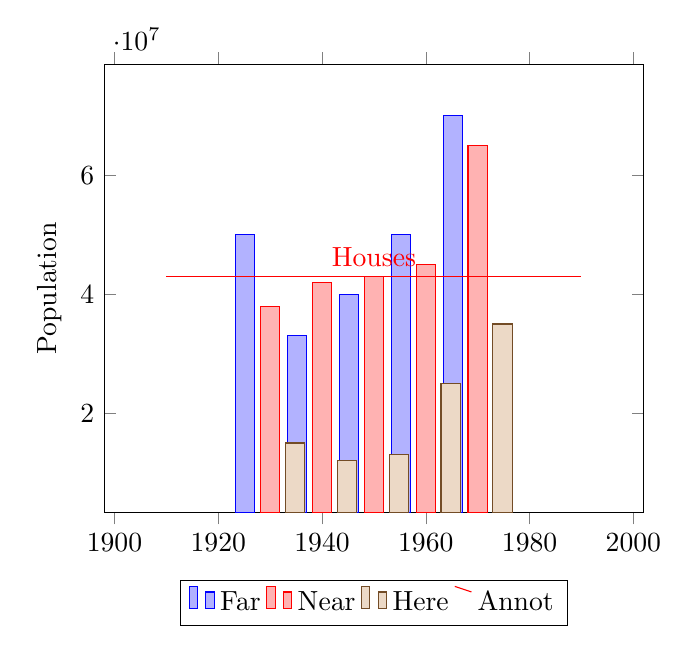
\begin{tikzpicture}
\begin{axis}[
	x tick label style={
		/pgf/number format/1000 sep=},
	ylabel=Population,
	enlargelimits=0.15,
	legend style={at={(0.5,-0.15)},
		anchor=north,legend columns=-1},
	ybar,
	bar width=7pt,
]
\addplot
	coordinates {(1930,50e6) (1940,33e6)
		(1950,40e6) (1960,50e6) (1970,70e6)};
\addplot
	coordinates {(1930,38e6) (1940,42e6)
		(1950,43e6) (1960,45e6) (1970,65e6)};
\addplot
	coordinates {(1930,15e6) (1940,12e6)
		(1950,13e6) (1960,25e6) (1970,35e6)};
\addplot[red,sharp plot,]
	coordinates {(1910,4.3e7) (1990,4.3e7)}
	node[above] at (axis cs:1950,4.3e7) {Houses};
\legend{Far,Near,Here,Annot}
\end{axis}
\end{tikzpicture}

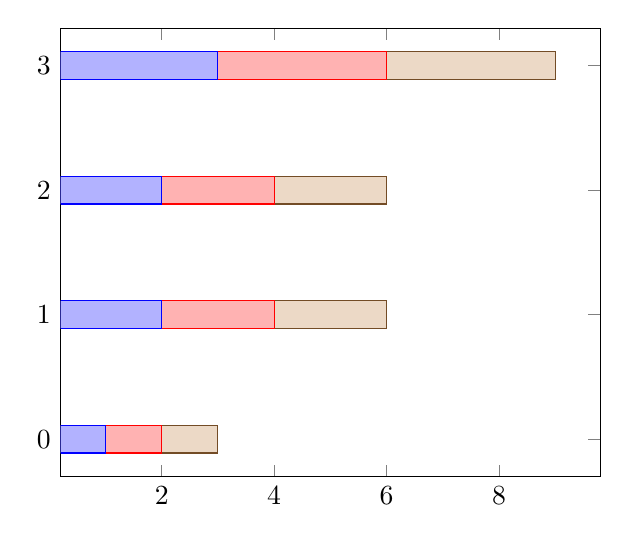
\begin{tikzpicture}
\begin{axis}[xbar stacked]
\addplot
	coordinates {(1,0) (2,1) (2,2) (3,3)};
\addplot
	coordinates {(1,0) (2,1) (2,2) (3,3)};
\addplot
	coordinates {(1,0) (2,1) (2,2) (3,3)};
\end{axis}
\end{tikzpicture}


	São considerados cursos de Matemática disciplinas que abordam as áreas do Cálculo, Álgebra Linear, Geometria, Vetores e Álgebra. Tais disciplinas são ministradas habitualmente pelos departamentos de Matemática das faculdades. A dificuldade é que em alguns casos os nomes das disciplinas, ou as próprias ementas, não representam o que de fato é ensinado. Todo o material curricular foi lido e classificações foram criadas para selecionar o que fato pode ser identificado como Matemática. 

	Os onze cursos de graduação em Ciência da Computação estudados foram escolhidos tendo como critério o fato de serem cursos de relevância nacional no Brasil na área de Computação, com resultados expressivos em rankings de avaliação de curso como o NOME COMPLETO ENADE em 2008 (por referencia)

	Um efeito colateral dessa escolha é que a maior parte dos programas estudados é de universidades públicas, o que deve ser levado em conta na análise dos dados uma vez que estes podem possuir ênfases diferenciadas na quantidade e abordagem de disciplinas de fundamentos (Matemática principalmente) em comparação a universidades particulares.

\section{Dados}
A tabela 1 apresenta o panorama geral das 11 universidades indicando seu tamanho e características do curso.

\begin{table*}
	\centering
	\caption{Some Typical Commands}
    \begin{tabular}{|c|c|c|c|c|c|}
        \hline
        Universidade  & Total créditos & Total horas & Período          & Graduação (anos) & Alunos por ano \\ \hline
        IME/USP[..]   & 199            & 2985        & Diurno           & 4               & 50                   \\ 
        PUC-RJ [..]   & 214            & 3212        & Diurno           & 4               & 50                   \\ 
        UFBA [..]     & 197            & 3347        & Diurno e Noturno & 4               & 90                   \\ 
        UFCG [..]     & 208            & 3120        & Diurno           & 4               & 90                   \\ 
        UFMG [..]     & 175            & 2625        & Diurno           & 4               & 80                   \\ 
        UFPE [..]     & 233            & 3495        & Diurno           & 4,5             & 100                  \\ 
        UFRGS [..]    & 196            & 3240        & Diurno           & 4,5             & 100                  \\ 
        UFRJ [..]     & 195            & 3075        & Diurno           & 4,5             & 50                   \\ 
        UFSC [..]     & 196            & 3528        & Diurno           & 4               & 100                  \\ 
        UNICAMP [..]  & 200            & 3000        & Noturno          & 5               & 50                   \\ 
        ICMC/USP [..] & 293            & 4395        & Diurno           & 5               & 100                  \\ 
        SBC [..]      & 160            & 2400        & N/A              & 4               & N/A                  \\ 
        SBC [..]      & 200            & 3000        & N/A              & 5               & N/A                  \\ 
        ACM [..]      & 280            & 4200        & N/A              & 4               & N/A                  \\
        \hline
    \end{tabular}
\end{table*}

	Nota-se que a maioria dos cursos são diurnos (Integrais), com duração entre 4 e 4,5 anos. É importante notar que a relação entre um crédito e as respectivas horas de aula varia entre universidades. Há cursos como os da da USP e o currículo de referência da ACM que consideram que um crédito equivale a 15 horas de aula, já o da UFSC, por exemplo, adota a relação 1 crédito = 18 horas. O currículo referência da SBC não indica qual é a relação adotada e assim os autores optaram por considerar o valor de 15 horas para fins de comparação.

	Na composição dos totais apresentados na tabela acima foram descritas as quantidades mínimas necessárias para a integralização curricular completa, abarcando créditos de disciplinas optativas e/ou estágios obrigatórios quando existem. 

	Analisando a coluna de total de horas podemos perceber que há uma grande variabilidade na quantidade exigida pelos currículos das diferentes universidades. Em média são exigidas 3177 h ($\sigma = 554 h $) para cursos de 4 anos, 3270 horas ($\sigma = 211 h$) para cursos de 4,5 anos e 3465 h ($\sigma = **** h$) para cursos de 5 anos.

	A tabela 2 trata especificamente dos conteúdos de Matemática. Aqui percebe-se uma grande diversidade na carga horária reservada a Matemática nos currículos dos cursos de Computação pelo Brasil. Aqui, as universidades possuem em média 15,6\% ($\sigma = 4,77 \%$) de disciplinas exclusivamente de desta área.

	Ainda, notamos que ao compararmos cada universidade com o currículo de referência da ACM (Que afirma ser o mínimo necessário para a cobertura do tópico) podemos verificar que 5 cursos possuem carga de Matemática maior ou igual que o recomendado e 6 cursos possuem menos. Isso corrobora a visão dos autores citados anteriormente que afirmam que Matemática é uma disciplina em decadência nos cursos de Computação.

\begin{table}
	\centering
	\caption{Some Typical Commands}
    \begin{tabular}{|c|c|c|}
        \hline
        Universidade & Créditos/horas Totais em Matemática & Créditos/horas Percentuais em Matemática \\ \hline
        IME/USP      & 50                                  & 25,10\%                                   \\ 
        UNICAMP      & 35                                  & 17,40\%                                   \\ 
        UFMG         & 19                                  & 10,80\%                                   \\ 
        UFRGS        & 24                                  & 12,00\%                                   \\ 
        UFRJ         & 31                                  & 21,20\%                                   \\ 
        PUC-RJ       & 22                                  & 10,20\%                                   \\ 
        ICMC/USP     & 36                                  & 16,50\%                                   \\ 
        UFPE         & 25                                  & 10,70\%                                   \\ 
        UFBA         & 32                                  & 16,20\%                                   \\ 
        UFSC         & 21                                  & 12,20\%                                   \\ 
        UFCG         & 28                                  & 13,40\%                                   \\ 
        SBC (4 anos) & 30                                  & 5,30\%                                    \\ 
        ACM          & 43                                  & 15,30\%                                   \\
        \hline
    \end{tabular}
\end{table}

\section{Conclusões}
	Neste artigo foi possível ver primeiramente como as disciplinas de Matemática são de grande importância para um futuro bacharel em Ciência da Computação. Foi visto que tal disciplina é uma base, que precisa ser sólida, para o desenvolvimento de tópicos mais avançados que se baseiam nela. Ainda, diversos educadores na área de Computação com artigos publicados em eventos de repercussão internacional compartilham desta tese.
	
	Por outro lado, foi constatado que esta área está sofrendo uma decadência em sua relevância, em parte pelo surgimento de diversas novas tendências no mercado de Computação que são absorvidas nos currículos dos cursos de graduação.
	
	Por fim, foi feita uma análise da situação atual da ênfase dada a Matemática nos currículos de 11 universidades brasileiras através de análises da carga horária absoluta e relativa. Foi constatado que mais de 50\% das universidades pesquisadas possuem uma carga menor que o recomendado pela ACM em seu currículo de referência.

% An example of a floating figure using the graphicx package.
% Note that \label must occur AFTER (or within) \caption.
% For figures, \caption should occur after the \includegraphics.
% Note that IEEEtran v1.7 and later has special internal code that
% is designed to preserve the operation of \label within \caption
% even when the captionsoff option is in effect. However, because
% of issues like this, it may be the safest practice to put all your
% \label just after \caption rather than within \caption{}.
%
% Reminder: the "draftcls" or "draftclsnofoot", not "draft", class
% option should be used if it is desired that the figures are to be
% displayed while in draft mode.
%
%\begin{figure}[!t]
%\centering
%\includegraphics[width=2.5in]{myfigure}
% where an .eps filename suffix will be assumed under latex, 
% and a .pdf suffix will be assumed for pdflatex; or what has been declared
% via \DeclareGraphicsExtensions.
%\caption{Simulation Results}
%\label{fig_sim}
%\end{figure}

% Note that IEEE typically puts floats only at the top, even when this
% results in a large percentage of a column being occupied by floats.


% An example of a double column floating figure using two subfigures.
% (The subfig.sty package must be loaded for this to work.)
% The subfigure \label commands are set within each subfloat command, the
% \label for the overall figure must come after \caption.
% \hfil must be used as a separator to get equal spacing.
% The subfigure.sty package works much the same way, except \subfigure is
% used instead of \subfloat.
%
%\begin{figure*}[!t]
%\centerline{\subfloat[Case I]\includegraphics[width=2.5in]{subfigcase1}%
%\label{fig_first_case}}
%\hfil
%\subfloat[Case II]{\includegraphics[width=2.5in]{subfigcase2}%
%\label{fig_second_case}}}
%\caption{Simulation results}
%\label{fig_sim}
%\end{figure*}
%
% Note that often IEEE papers with subfigures do not employ subfigure
% captions (using the optional argument to \subfloat), but instead will
% reference/describe all of them (a), (b), etc., within the main caption.


% An example of a floating table. Note that, for IEEE style tables, the 
% \caption command should come BEFORE the table. Table text will default to
% \footnotesize as IEEE normally uses this smaller font for tables.
% The \label must come after \caption as always.
%
%\begin{table}[!t]
%% increase table row spacing, adjust to taste
%\renewcommand{\arraystretch}{1.3}
% if using array.sty, it might be a good idea to tweak the value of
% \extrarowheight as needed to properly center the text within the cells
%\caption{An Example of a Table}
%\label{table_example}
%\centering
%% Some packages, such as MDW tools, offer better commands for making tables
%% than the plain LaTeX2e tabular which is used here.
%\begin{tabular}{|c||c|}
%\hline
%One & Two\\
%\hline
%Three & Four\\
%\hline
%\end{tabular}
%\end{table}


% Note that IEEE does not put floats in the very first column - or typically
% anywhere on the first page for that matter. Also, in-text middle ("here")
% positioning is not used. Most IEEE journals/conferences use top floats
% exclusively. Note that, LaTeX2e, unlike IEEE journals/conferences, places
% footnotes above bottom floats. This can be corrected via the \fnbelowfloat
% command of the stfloats package.



\section{Conclusion}
The conclusion goes here.




% conference papers do not normally have an appendix


% use section* for acknowledgement
\section*{Acknowledgment}


The authors would like to thank...





% trigger a \newpage just before the given reference
% number - used to balance the columns on the last page
% adjust value as needed - may need to be readjusted if
% the document is modified later
%\IEEEtriggeratref{8}
% The "triggered" command can be changed if desired:
%\IEEEtriggercmd{\enlargethispage{-5in}}

\bibliographystyle{IEEEtran}
\bibliography{bibliography}


\end{document}

